\documentclass[runningheads]{llncs}

\pdfminorversion=7

\usepackage[T1]{fontenc}
\usepackage{graphicx}
\usepackage{booktabs}
\usepackage{array}
\usepackage{amsmath}
\usepackage{amssymb}
\usepackage{url}

\setlength{\textfloatsep}{8pt plus 1pt minus 2pt}
\setlength{\floatsep}{6pt plus 1pt minus 1pt}
\setlength{\intextsep}{6pt plus 1pt minus 1pt}
\setlength{\abovecaptionskip}{4pt}
\setlength{\belowcaptionskip}{2pt}
\providecommand{\doi}[1]{DOI:\ \texttt{\detokenize{#1}}}
\renewcommand{\doi}[1]{DOI:\ \texttt{\detokenize{#1}}}
\renewcommand{\url}[1]{}
\providecommand{\urlprefix}{}
\renewcommand{\urlprefix}{}

\title{BotRHG: Reliability-Guided Hypergraph Learning for Social Bot Detection}
\titlerunning{BotRHG for Social Bot Detection}

\author{Anonymous Author(s)}
\authorrunning{Anonymous Author(s)}
\institute{Anonymous Institution}

\begin{document}

\maketitle

\begin{abstract}
Malicious social bots manipulate online discourse by spreading misinformation, amplifying coordinated opinions, and undermining trust in social platforms. Recent graph-based detectors exploit account attributes and relational structure, but they rarely consider when a detector's prediction should be trusted. To address this limitation, we propose BotRHG, a reliability-guided hypergraph learning framework that uses a local reliability estimate to route low-reliability accounts and activates selective residual correction only for routed accounts. Experiments demonstrate that our approach achieves state-of-the-art performance on two Twitter bot detection benchmarks. Additional studies validate the robustness and effectiveness of each component of our method.

\keywords{Social bot detection \and hypergraph learning \and reliability estimation \and higher-order networks}
\end{abstract}

\section{Introduction}\label{sec:introduction}

Online social networks (OSNs), such as Twitter/X, Facebook, and Weibo, have become important infrastructures for information sharing and public discussion. Social bots are automated or semi-automated accounts that mimic human behavior and interact with users at scale~\cite{ferrara2016rise}. Malicious bots can spread misinformation, amplify coordinated opinions, invade privacy, and manipulate online topics, making reliable social bot detection an important task~\cite{feng2021twibot20,twibot22benchmark}.

Social bot detection has shifted from handcrafted feature engineering to representation learning over social graphs. Early detectors used metadata, activity patterns, network statistics, and tweet content with conventional classifiers~\cite{davis2016botornot,varol2017online,bot_hunter2018,friendbot2020}, but observable profile and content signals are vulnerable to adaptive manipulation and content imitation~\cite{cresci2017paradigm}. Recent methods therefore exploit account attributes, text, and social relations: heterogeneous graph detectors model relation-specific interactions~\cite{feng2021botrgcn,feng2022rgt}; text--graph and multimodal methods fuse textual and structural evidence~\cite{lei2023bic,liu2023botmoe,zhou2024lgb}; reliability-aware approaches reduce noisy or heterophilous edges~\cite{qiao2025bece,lin2025botbr}; and higher-order methods capture group-wise relations beyond pairwise links~\cite{gao2025higherorder,yang2024sebot}. These studies strengthen detector representations, but they leave a complementary question underexplored: how to estimate node-level prediction reliability and determine when a detector's prediction should be trusted.

To address this gap, we propose BotRHG, a reliability-guided hypergraph learning framework for social bot detection. A base detector provides initial node-level decisions, a local reliability estimate identifies low-reliability accounts, and a hypergraph supplies higher-order evidence only for routed accounts. For routed accounts, selective residual correction fuses the base representation with hypergraph evidence from semantically or structurally related users; for non-routed accounts, the base prediction is preserved.

Our experiments on TwiBot-20 and TwiBot-22 demonstrate that the proposed method achieves state-of-the-art performance, outperforming eight competitive social bot detection baselines. Extensive analyses further validate the effectiveness of reliability-guided routing and selective residual correction, and show that selective higher-order evidence can improve the detection of low-reliability accounts.

The main contributions of this work are summarized as follows:
\begin{enumerate}
\item We propose BotRHG, a reliability-guided hypergraph learning framework for social bot detection, using node-level prediction reliability to guide selective higher-order learning.
\item We develop a reliability-guided correction module that converts local reliability estimates into account-level routing decisions and performs selective residual fusion over support hyperedges, enabling targeted higher-order correction while preserving reliable base predictions.
\item Our experiments show that the proposed method achieves state-of-the-art performance on two widely used Twitter bot benchmarks. Extensive analyses further validate the effectiveness and robustness of our approach.
\end{enumerate}

\section{Related Work}\label{sec:related}

Social bot detection has evolved from handcrafted feature engineering to graph-based representation learning and, more recently, reliability-aware modeling. Early methods relied on observable account, activity, network, and content signals, such as BotOrNot, online human--bot interaction modeling, Bot-Hunter, and FriendBot~\cite{davis2016botornot,varol2017online,bot_hunter2018,friendbot2020}, but these approaches remain vulnerable to feature manipulation and content imitation~\cite{cresci2017paradigm}. With the release of the TwiBot benchmarks~\cite{feng2021twibot20,twibot22benchmark}, graph-based methods increasingly exploited heterogeneous social relations as structural evidence for bot detection. Representative models include BotRGCN~\cite{feng2021botrgcn}, RGT~\cite{feng2022rgt}, and BIC~\cite{lei2023bic}, which improve account classification through relational propagation and text--graph interaction. Since pairwise edges may not fully capture coordinated behavior, recent work has further introduced higher-order relation modeling, for example by constructing hyperedges from neighborhood differences~\cite{shi2024hypergraphbot} or jointly modeling pairwise, hop-wise, and group-wise relations~\cite{gao2025higherorder}; however, noisy hypergraphs may also introduce task-irrelevant connections~\cite{cai2022hypergraphstructure}. More recent studies have begun to emphasize reliability in social bot detection. BECE estimates edge confidence to suppress unreliable graph evidence~\cite{qiao2025bece}, BotBR combines balanced feature fusion with reliability-enhanced graph learning~\cite{lin2025botbr}, and BotPercent calibrates model outputs for community-level bot-population estimation rather than node-level prediction correction~\cite{tan2023botpercent}. In contrast, our method uses a calibration-inspired local reliability estimate to guide selective higher-order correction for individual accounts.

\section{Methodology}\label{sec:method}

Figure~\ref{fig:selective_residual_framework} illustrates the proposed BotRHG framework. The framework first encodes each account into textual and property representations, then constructs hyperedges from local reference neighbors, and finally applies selective residual correction only to routed accounts with lower local reliability.

\begin{figure}[!htbp]
    \centering
    \includegraphics[width=.88\textwidth]{figures/Architecture.pdf}
    \caption{Framework of BotRHG. The model constructs account representations, builds hyperedges from local reference neighbors, and activates selective residual correction only for routed accounts.}
    \label{fig:selective_residual_framework}
\end{figure}

\subsection{Preliminaries and Problem Formulation}\label{sec:preliminaries}

Let $G_{\mathrm{rel}}=(V,E_{\mathrm{rel}},\mathcal{R},X)$ denote a multi-relation social graph, where $V$ is the account set, $E_{\mathrm{rel}}$ the observed social relations, $\mathcal{R}$ the relation types, and $X\in\mathbb{R}^{|V|\times d}$ the account feature matrix. Each labeled account has $y_i\in\{0,1\}$, where $0$ denotes human and $1$ denotes bot.

We consider a trained base detector $f_{\mathrm{base}}$ that produces an initial posterior $p_i=f_{\mathrm{base}}(x_i,G_{\mathrm{rel}})$, a base prediction $\hat{y}^{(0)}_i=\arg\max_c p_i^{(c)}$, and a low-order representation $x_{\mathrm{low},i}$. Our goal is not to replace the base detector for all accounts, but to identify base predictions with lower local reliability and refine them with higher-order evidence.

\subsection{Feature Encoder}

The feature encoder converts heterogeneous account information into textual and property features.

\paragraph{Textual encoder.}
For each Twitter account, we have access to profile metadata, the self-description, and recent tweets. To obtain a unified user representation compatible with the language model encoder, we linearize these heterogeneous user attributes into a single textual sequence. Specifically, we organize the profile metadata as a profile segment and concatenate it with the description and tweet segments:
\begin{equation}
s_i=\texttt{[P]}\ \mathrm{profile}_i\ \texttt{[D]}\ \mathrm{description}_i\ \texttt{[T]}\ \mathrm{tweets}_i ,
\label{eq:text-sequence}
\end{equation}
Here, \texttt{[P]}, \texttt{[D]}, and \texttt{[T]} denote special segment markers for profile metadata, description, and tweets, respectively. Mentions, hashtags, and URLs are normalized as \texttt{@USER}, \texttt{\#HASHTAG}, and \texttt{HTTPURL}.

\begin{figure}[!htbp]
    \centering
    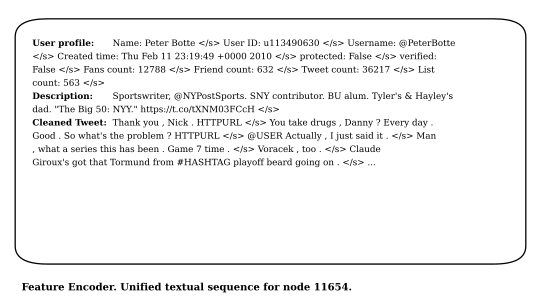
\includegraphics[width=.76\textwidth,trim=75 130 180 60,clip]{figures/feature encoder.pdf}
    \caption{Unified user textual sequence used by the feature encoder.}
    \label{fig:user_text_sequence}
\end{figure}

Following recent language-model-based bot detectors~\cite{cai2024lmbot,zhou2024lgb}, we encode the resulting sequence with a fine-tuned RoBERTa model to obtain the textual representation $h_i^{\mathrm{text}}$, and stack all account representations to form $X^{\mathrm{text}}$.

\paragraph{Property encoder.}
Besides the unified textual sequence, we retain structured user properties to capture account-level and social statistics that are complementary to textual semantics. Following prior bot detection studies~\cite{davis2016botornot,varol2017online,lin2025botbr,gao2025higherorder}, we extract profile, activity, and network-structure attributes from raw user data, and organize them into numerical and categorical feature groups, denoted by $X_{\mathrm{num}}$ and $X_{\mathrm{cat}}$, respectively. Continuous attributes in $X_{\mathrm{num}}$ are normalized with training-split statistics, while categorical and Boolean attributes in $X_{\mathrm{cat}}$ are converted into indicator features. We then project them into latent property representations through two feed-forward layers with LeakyReLU activation $\phi$:
\begin{align}
X_n &= \phi(X_{\mathrm{num}}W_n+b_n),
\label{eq:numerical-property-projection}\\
X_c &= \phi(X_{\mathrm{cat}}W_c+b_c),
\label{eq:categorical-property-projection}
\end{align}
where $W_n$, $W_c$, $b_n$, and $b_c$ are learnable parameters. The initial node feature matrix is
\begin{equation}
X_{\mathrm{in}} = X^{\mathrm{text}} \Vert X_n \Vert X_c ,
\label{eq:node-feature}
\end{equation}
and we denote its $i$-th row by $x_i$.

\subsection{Hypergraph Construction}

To build higher-order evidence, we combine the low-order representation from the base detector with the node feature representation:
\begin{equation}
x_{\mathrm{new},i}=x_{\mathrm{low},i}\Vert x_i .
\label{eq:hybrid-representation}
\end{equation}
Stacking all account representations gives $X_{\mathrm{new}}$, which is used for hypergraph construction.

Let $\mathcal{T}$ denote the target accounts and let $\mathcal{U}_{\mathrm{ref}}$ denote the reference pool used for hypergraph construction and reliability estimation. Following the standard split protocol, reference neighbors are retrieved from the corresponding reference pool, and the target account itself is excluded from its neighborhood. For each target account, we construct a candidate hyperedge from local reference neighbors:
\begin{equation}
e_i=\{i\}\cup \mathcal{N}^{\mathrm{support}}_k(i),\qquad i\in \mathcal{T},
\label{eq:support-hyperedge}
\end{equation}
where $\mathcal{N}^{\mathrm{support}}_k(i)\subseteq \mathcal{U}_{\mathrm{ref}}\setminus\{i\}$ contains the $k$ nearest reference accounts in $X_{\mathrm{new}}$. These target-centered hyperedges provide candidate higher-order evidence for subsequent selective correction.

\subsection{Reliability-Guided Selective Correction}

The correction module is selective: it preserves the base prediction for most accounts and activates higher-order correction only when local reference evidence indicates lower local reliability.

\paragraph{Local reliability estimation.}
Inspired by local reference comparison in conformal-style methods~\cite{vovk2005algorithmic} and selective prediction~\cite{geifman2017selective}, we estimate the reliability of each base prediction relative to similar reference accounts through local reliability estimation inspired by confidence calibration and local reference comparison. We first define the confidence deficit of account $i$ as
\begin{equation}
u_i=1-\max_c p_i^{(c)}.
\label{eq:confidence-deficit}
\end{equation}
For a reference account $j$, let $s_{ij}$ denote the cosine similarity in $X_{\mathrm{new}}$. We convert it to angular distance $d_{ij}=\sqrt{\max(0,2-2s_{ij})}$ and weight $w_{ij}=\exp(-d_{ij}/\lambda)$, where $\lambda=1.0$. The local reference comparison yields
\begin{equation}
\tau_i =
    \frac{1+\sum_{j\in\mathcal{U}_{\mathrm{ref}}\setminus\{i\}} w_{ij}\mathbb{I}[u_j\ge u_i]}
         {1+\sum_{j\in\mathcal{U}_{\mathrm{ref}}\setminus\{i\}} w_{ij}},
\quad
\rho_i = \tau_i,
\quad
r_i = 1-\rho_i .
\label{eq:local-reference-score}
\end{equation}
Eq.~\eqref{eq:local-reference-score} defines the local reliability estimate $\rho_i$ and the corresponding correction risk $r_i$. Accounts that are more uncertain than their local references receive lower reliability and higher correction risk.

\paragraph{Reliability-guided routing.}
Given a routing budget $\beta$, we select
\begin{equation}
B=\lfloor \beta |\mathcal{T}| \rfloor
\label{eq:routing-budget}
\end{equation}
accounts with the highest correction risk:
\begin{align}
R_{\beta} &= \operatorname{TopB}(\{r_i\}_{i\in \mathcal{T}}, B),
\label{eq:routed-set}\\
\mathcal{E}_H^{\beta} &= \{e_i\mid i\in R_{\beta}\}.
\label{eq:routed-hyperedges}
\end{align}
Based on the routing budget in Eq.~\eqref{eq:routing-budget}, Eqs.~\eqref{eq:routed-set} and~\eqref{eq:routed-hyperedges} select the routed account set and the corresponding routed hyperedges. This reliability-guided routing strategy treats higher-order reasoning as a selective intervention, allowing the model to preserve reliable base predictions while concentrating additional correction on low-reliability accounts.

\paragraph{Selective residual correction.}
Let $H\in\{0,1\}^{|V|\times |\mathcal{E}_H^{\beta}|}$ be the incidence matrix of the routed hyperedges. Eqs.~\eqref{eq:hypergraph-initialization} and~\eqref{eq:hypergraph-propagation} compute higher-order representations from $X_{\mathrm{new}}$ through hypergraph propagation:
\begin{align}
X_H^{(0)} &= X_{\mathrm{new}} W_0,
\label{eq:hypergraph-initialization}\\
X_H^{(\ell+1)} &=
\phi\!\left(D_v^{-1/2} H D_e^{-1} H^\top D_v^{-1/2} X_H^{(\ell)} W_{\ell}\right),
\label{eq:hypergraph-propagation}
\end{align}
where $D_v$ and $D_e$ are the node and hyperedge degree matrices, and $\phi(\cdot)$ is a nonlinear activation. The resulting representation is denoted by $x_{\mathrm{high},i}$.

For each routed account, selective residual correction is defined in Eqs.~\eqref{eq:residual-update} and~\eqref{eq:residual-correction} as
\begin{align}
\delta_i &= \psi(x_{\mathrm{low},i}\Vert x_{\mathrm{high},i}),
\label{eq:residual-update}\\
h_i &= x_{\mathrm{low},i}+m_i\delta_i,
\label{eq:residual-correction}
\end{align}
where $\psi$ is a learnable residual projection and $m_i=\mathbb{I}[i\in R_{\beta}]$. The corrected posterior is
\begin{equation}
q_i=\operatorname{softmax}(W_c h_i+b_c),\qquad i\in R_{\beta}.
\label{eq:corrected-posterior}
\end{equation}
The final prediction follows the selective rule in Eq.~\eqref{eq:final-prediction}
\begin{equation}
\hat{y}_i=
\begin{cases}
\arg\max_c q_i^{(c)}, & i\in R_{\beta},\\
\hat{y}^{(0)}_i, & i\notin R_{\beta}.
\end{cases}
\label{eq:final-prediction}
\end{equation}

\subsection{Training and Inference}

Following the standard benchmark split, the base detector is trained with supervised classification and then fixed. During correction training, only the hypergraph branch, the residual projection $\psi$, and the classifier parameters $(W_c,b_c)$ are optimized with cross-entropy on routed training accounts.

At inference time, the fixed base detector produces $p_i$, $\hat{y}^{(0)}_i$, and $x_{\mathrm{low},i}$; hyperedges are constructed from the corresponding reference pool without using target labels; and selective residual correction is applied only to routed accounts, while non-routed accounts retain the base prediction.

\section{Experiments}\label{sec:experiments}

The experiments evaluate whether BotRHG improves social bot detection and how its key components affect performance. We first describe the experimental setup, and then present the main comparison, component analysis, hyperparameter sensitivity, and a case study.

\subsection{Experiment Setup}

\paragraph{Datasets.}
We use two public social bot detection benchmarks, TwiBot-22~\cite{twibot22benchmark} and TwiBot-20~\cite{feng2021twibot20}. TwiBot-20 contains 5,237 human accounts, 6,589 bot accounts, 229,580 nodes, and 227,979 normalized social edges; we adopt the standard setting in~\cite{feng2021twibot20}. For TwiBot-22, we conduct evaluation on a fixed sampled subset. The subset is sampled within the released train/validation/test splits and is kept identical for all compared methods. It contains 11,542 labeled accounts, including 1,575 bots and 9,967 humans, together with 128,095 social edges.

\paragraph{Baselines.}
Baselines cover four representative groups. Feature-based methods include BotHunter~\cite{bot_hunter2018} and FriendBot~\cite{friendbot2020}. Graph-based and multimodal detectors include BotRGCN~\cite{feng2021botrgcn}, RGT~\cite{feng2022rgt}, BIC~\cite{lei2023bic}, BotMoE~\cite{liu2023botmoe}, and SEBot~\cite{yang2024sebot}. We also compare with BotBR~\cite{lin2025botbr}, a reliability-oriented detector, and LMBot variants~\cite{cai2024lmbot} for graph-knowledge distillation and graph-less inference.

\paragraph{Evaluation metrics.}
Following prior studies~\cite{feng2022rgt,yang2024sebot,gao2025higherorder}, we report Accuracy, Precision, and F1-score. Precision and F1-score are macro-averaged. In the result tables, bold and underlined values indicate the best and second-best performance, respectively.

\paragraph{Implementation details.}
For the main comparison, we report the mean and standard deviation over five runs. Ablation and hyperparameter sensitivity experiments are conducted on TwiBot-20 under a fixed random seed setting. All textual, profile, behavioral, and graph-based features are normalized using training-set statistics. The hidden dimension is set to 788, and the graph and hypergraph modules are configured with two layers. We perform grid search over the KNN support size $K \in \{4,8,16\}$, sampled fanout $\in \{32,64,128\}$, and routing budget $\beta \in \{5\%,10\%,20\%\}$, with $K=8$, fanout 64, and $\beta=10\%$ used as the default setting. Graph training runs for at most 200 steps with a GNN batch size of 512. We use AdamW for optimization, with learning rates of $1\times10^{-5}$ for the text encoder and $5\times10^{-4}$ for graph modules, and apply graph-side weight decay of $1\times10^{-5}$. The experiments are implemented with PyTorch, PyTorch Geometric, and scikit-learn, and conducted on a CentOS 7 server equipped with two NVIDIA GeForce RTX 3090 GPUs.

\subsection{Main Results}

Table~\ref{tab:main-results} compares the proposed detector with representative baselines. All main results are reported as the mean and standard deviation over five runs.

\begin{table}[t]
\caption{Main results on TwiBot-20 and sampled TwiBot-22. Values are reported as percentages. Bold and underlined values indicate the best and second-best results, respectively. A dash denotes unavailable compatible results.}
\label{tab:main-results}
\centering
\scriptsize
\setlength{\tabcolsep}{2.5pt}
\resizebox{\textwidth}{!}{
\begin{tabular}{m{2.2cm}|cccccc}
\toprule
Method & \multicolumn{3}{c}{TwiBot-20} & \multicolumn{3}{c}{TwiBot-22} \\
\cmidrule(lr){2-4}\cmidrule(lr){5-7}
 & Accuracy & Precision & F1-score & Accuracy & Precision & F1-score \\
\midrule
BotHunter~\cite{bot_hunter2018} & 75.28 $\pm$ 0.42 & 76.34 $\pm$ 0.51 & 74.39 $\pm$ 0.42 & 77.31 $\pm$ 0.19 & \textbf{78.56 $\pm$ 1.19} & 63.23 $\pm$ 0.31 \\
FriendBot~\cite{friendbot2020} & 77.19 $\pm$ 0.46 & 77.71 $\pm$ 0.46 & 76.63 $\pm$ 0.48 & -- & -- & -- \\
\midrule
BotRGCN~\cite{feng2021botrgcn} & 85.68 $\pm$ 0.57 & 85.88 $\pm$ 0.69 & 85.49 $\pm$ 0.55 & 72.21 $\pm$ 2.29 & 66.50 $\pm$ 4.57 & 60.55 $\pm$ 2.10 \\
RGT~\cite{feng2022rgt} & 86.39 $\pm$ 0.25 & 86.63 $\pm$ 0.26 & 86.20 $\pm$ 0.26 & 72.24 $\pm$ 2.38 & 64.40 $\pm$ 5.58 & 56.73 $\pm$ 6.91 \\
BIC~\cite{lei2023bic} & 85.55 $\pm$ 0.50 & 85.78 $\pm$ 0.53 & 85.34 $\pm$ 0.51 & \underline{78.56 $\pm$ 0.97} & \underline{74.33 $\pm$ 1.40} & \textbf{73.42 $\pm$ 0.95} \\
BotMoE~\cite{liu2023botmoe} & 86.12 $\pm$ 0.50 & 86.38 $\pm$ 0.66 & 85.92 $\pm$ 0.47 & 64.99 $\pm$ 1.60 & 65.62 $\pm$ 0.92 & 63.64 $\pm$ 1.36 \\
SEBot~\cite{yang2024sebot} & 86.29 $\pm$ 0.33 & 86.52 $\pm$ 0.31 & 86.10 $\pm$ 0.35 & -- & -- & -- \\
\midrule
BotBR~\cite{lin2025botbr} & \underline{86.91 $\pm$ 0.20} & 87.19 $\pm$ 0.21 & \underline{86.72 $\pm$ 0.21} & 76.09 $\pm$ 3.99 & 68.94 $\pm$ 17.60 & 60.34 $\pm$ 12.20 \\
\midrule
LMBot-GNN~\cite{cai2024lmbot} & 85.11 $\pm$ 0.39 & 86.44 $\pm$ 0.73 & 84.65 $\pm$ 0.39 & 74.98 $\pm$ 1.46 & 69.19 $\pm$ 2.42 & 64.29 $\pm$ 3.80 \\
LMBot-LM~\cite{cai2024lmbot} & 85.41 $\pm$ 0.10 & \underline{87.47 $\pm$ 0.57} & 84.87 $\pm$ 0.21 & 74.72 $\pm$ 1.27 & 69.46 $\pm$ 2.80 & 62.90 $\pm$ 2.25 \\
\midrule
\textbf{BotRHG} & \textbf{88.93 $\pm$ 0.53} & \textbf{89.18 $\pm$ 0.43} & \textbf{88.78 $\pm$ 0.48} & \textbf{82.41 $\pm$ 1.40} & 73.14 $\pm$ 1.34 & \underline{71.31 $\pm$ 1.04} \\
\bottomrule
\end{tabular}
}
\end{table}


Our method achieves the best performance on TwiBot-20 across Accuracy, Precision, and F1-score, outperforming the strongest baseline BotBR by 2.02, 1.99, and 2.06 percentage points, respectively. On TwiBot-22, it obtains the highest Accuracy and a competitive F1-score, ranking second to BIC on F1-score. These results show that BotRHG improves the standard TwiBot-20 benchmark and remains effective on the TwiBot-22 setting. FriendBot and SEBot are not included for direct comparison on TwiBot-22 because compatible results are not available under the same evaluation protocol.

Feature-based methods such as BotHunter and FriendBot rely heavily on handcrafted profile, content, and network statistics, and their performance is limited when bots imitate observable account attributes. Graph-based and multimodal methods, including BotRGCN, RGT, BIC, BotMoE, SEBot, and BotBR, exploit relational or heterogeneous evidence and generally perform better than feature-only baselines. However, they usually apply structural propagation or feature fusion uniformly. In contrast, our method uses a local reliability estimate for each account and introduces higher-order hypergraph evidence only through reliability-guided routing and selective residual correction, which helps preserve reliable base predictions while improving low-reliability accounts.

\subsection{Ablation Study}

To examine the contribution of each component, we construct four variants of the proposed model. \textit{w/o Reliability-Guided Routing} removes reliability-guided routing and applies correction without account-level reliability selection. \textit{w/o Residual Correction} keeps the routing stage but disables the selective residual correction module. \textit{w/o Hypergraph Correction} replaces hypergraph correction with a fine-tuned RoBERTa + RGCN variant, comparing the proposed design with a conventional graph detector. \textit{w/o Random Routing} randomly selects the same number of routed accounts under the same routing budget, replacing the routing induced by the local reliability estimate with random routing.

\begin{table}[t]
\caption{Ablation study on TwiBot-20. The full model uses $K=8$, fanout 64, and a routing budget of 10\%.}
\label{tab:component-ablation}
\centering
\small
\begin{tabular}{lcc}
\toprule
Variant & Accuracy & F1-score \\
\midrule
Full model & \textbf{0.8893} & \textbf{0.8878} \\
w/o Reliability-Guided Routing & 0.8850 & 0.8835 \\
w/o Residual Correction & 0.8774 & 0.8755 \\
w/o Hypergraph Correction & 0.8715 & 0.8684 \\
w/o Random Routing & 0.8698 & 0.8677 \\
\bottomrule
\end{tabular}
\end{table}


Table~\ref{tab:component-ablation} reports the fixed-seed component analysis on TwiBot-20. The full model achieves the best Accuracy and F1-score. Removing reliability-guided routing reduces F1-score from 0.8878 to 0.8835, indicating that reliability-guided routing helps identify accounts that benefit from additional correction. Removing selective residual correction causes a larger drop to 0.8755, suggesting that higher-order correction provides useful information beyond the base detector. The strongest degradations come from w/o Hypergraph Correction and w/o Random Routing, whose F1-scores fall to 0.8684 and 0.8677, respectively. These results suggest that the improvement does not come merely from adding graph capacity or correcting a fixed number of accounts; it depends on both selective residual correction and routing based on the local reliability estimate.

\subsection{Hyperparameter Sensitivity}

We examine three hyperparameters under the fixed-seed TwiBot-20 setting: the KNN support size $K$, the sampled fanout, and the routing budget $\beta$. Figure~\ref{fig:hparam-sensitivity} reports the results.

\begin{figure}[!htbp]
    \centering
    \includegraphics[width=.92\textwidth]{figures/twibot20_seed1_hparam_sensitivity.pdf}
    \caption{Hyperparameter sensitivity on TwiBot-20. The dashed line indicates the full-model setting: $K=8$, fanout 64, and a routing budget of 10\%.}
    \label{fig:hparam-sensitivity}
\end{figure}

For the KNN support size, the model performs best at $K=8$. A smaller support set may provide insufficient local reference evidence, while a larger support set may include weakly related accounts and dilute the reliability signal. For sampled fanout, fanout 64 gives the best result, and fanout 32 remains competitive, whereas fanout 128 leads to a clear performance drop. This trend indicates that expanding the sampled neighborhood can enrich structural context, but excessive expansion may introduce noisy or task-irrelevant relations. For the routing budget, $\beta=10\%$ achieves the best Accuracy and F1-score. A smaller budget may miss low-reliability accounts, while a larger budget routes more accounts whose base predictions are already reliable, increasing unnecessary correction.

\subsection{Case Study}

\begin{figure}[!t]
    \centering
    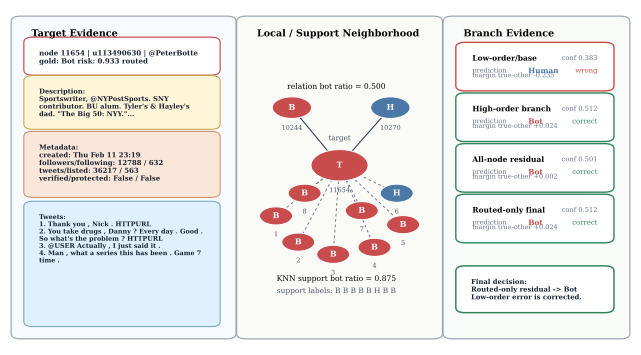
\includegraphics[width=.56\textwidth,trim=145 165 510 125,clip]{figures/casestudy.pdf}
    \caption{Case study for an initially misclassified routed account on TwiBot-20. Solid lines denote observed social neighbors, and dashed lines denote higher-order KNN links used for selective residual correction.}
    \label{fig:case-study}
\end{figure}

Figure~\ref{fig:case-study} presents a bot account that is initially misclassified as Human by the base detector. Its profile and tweet content do not exhibit clear bot-specific signals, and its observed social neighborhood contains both human and bot accounts, making the low-order prediction biased toward the Human class. After reliability-guided routing, the dashed KNN links associate the target account with bot-related reference accounts in the hybrid representation space and form a hyperedge. Selective residual correction then introduces additional higher-order evidence, increases the confidence toward the Bot class, and revises the incorrect prediction.

\section{Conclusion}

We study BotRHG for social bot detection. The proposed method uses a local reliability estimate, obtained through a calibration-inspired local reliability estimation process, to guide selective correction with higher-order evidence. Experiments, ablation studies, and sensitivity analyses support the effectiveness of the method under the evaluated settings.

\paragraph{Limitations and Future Work.}
The current study is still limited by data coverage and performance constraints, and the method has not yet been fully extended to the complete TwiBot-22 setting. Although the present results support the usefulness of BotRHG, broader validation in more challenging settings is still needed. Future work will strengthen the semantic modeling ability of the framework by incorporating large language models to provide richer contextual and higher-order semantic knowledge, and will further explore how such semantic signals can improve reliability estimation and correction quality for social bot detection.


\renewcommand{\doi}[1]{DOI:\ \texttt{\detokenize{#1}}}
\renewcommand{\url}[1]{}
\renewcommand{\urlprefix}{}
\bibliographystyle{splncs04}
\bibliography{references}

\end{document}
